\chapter{Populaire samenvatting}

Vandaag de dag is men steeds meer bezig met het delen van informatie. Omdat het belangrijk is dat deze informatie ergens opgeslagen wordt, zijn we altijd op zoek naar \emph{compressie}: het `inpakken' van informatie zodat het minder ruimte in beslag neemt.

Bij deze compressie zijn twee types te onderscheiden. Bijvoorbeeld tekst moet na de compressie perfect ge\emph{reconstrueerd} kunnen worden. Dit soort signalen zullen wij niet behandelen. Wij zijn ge\"interesseerd in \emph{lossy} compressie, wat betekent dat we `oninteressante informatie' gewoon weg kunnen gooien met de hoop dat de reconstructie goed genoeg lijkt op het origineel.

In het bijzonder zullen wij ons vizier richten op beeldmateriaal, eerst stil en daarna bewegend. Foto's worden veelal opgeslagen in het zogenaamde JPEG-beeldformaat: \texttt{.jpg}. De wiskunde achter dit compressie-algoritme is niet triviaal en wij zullen hier dan ook grondig op ingaan in ons verslag. De Fouriertransformatie wordt in \emph{signaalverwerking} al honderden jaren toegepast om signalen (functies, geluid, foto's, films) te schrijven in een andere \emph{basis}, namelijk de basis van de complexe $e$-machten $e^{2 \pi i t}$. We hopen hierbij maar dat ons signaal goed te benaderen valt in deze basis: een klein aantal grote co\"effici\"enten en een groot aantal kleine.

Het lot wil dat dit helemaal niet altijd goed werkt, de Fouriertransformatie werkt namelijk niet goed wanneer een afbeelding harde randen heeft.
Daarm is er in de laatste dertig jaar een nieuwe speler op het gebied van signaalverwerking opgedoken, de \mbox{\emph{Wavelettransformatie}}. 
We spreken dan over een nieuwe versie van JPEG: JPEG-2000.
 
De wavelettransformatie maakt gebruik van de wavelet, een r\"eele functie waarvoor geldt dat $\int_{-\infty}^\infty \psi(t) dt = 0$;
deze heeft dus net als een golf even hoge pieken als dalen, vanwaar de naam.
Dit op zich is nog niet handig, maar er zijn wavelets met een zogenaamde \emph{compacte drager}:
de functie is identiek $0$ buiten een \emph{begrensd} en \emph{gesloten} gebied. 
Hierin ligt dan het verschil met de complexe $e$-machten van de Fouriertransformatie, waarvan de drager gelijk is aan $\R$. 
Het effect van deze compacte drager is nu dat niet elke wavelet last heeft van een harde rand in het plaatje, maar slechts een deel van de functies.
Zie figuur \ref{fig:samenv}.voor twee van de wavelets die we gebruikt hebben.

\begin{figure}[h]
  \centering
  \begin{subfigure}{0.48\linewidth}
    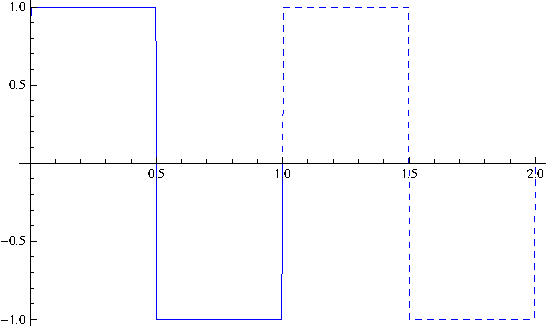
\includegraphics[width=\linewidth]{plaatjes/db1.pdf}
  \end{subfigure}
  \begin{subfigure}{0.48\linewidth}
    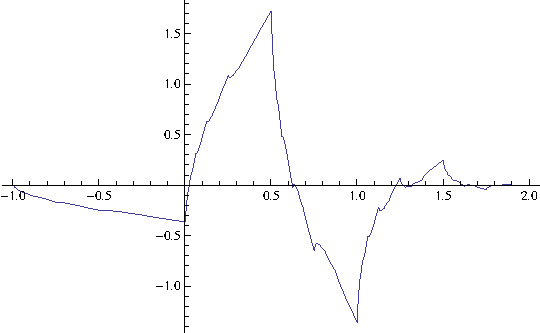
\includegraphics[width=\linewidth]{plaatjes/db2_psi.pdf}
  \end{subfigure}
  \caption{Links: De Haarwavelet. Rechts: De Daubechies-2 wavelet.}
\label{fig:samenv}
\end{figure}

Een orthogonale waveletbasis is nu een verzameling $\{ \psi_{j,n}: j \in \N_0,\, n \in \Z \}$ waarbij de basisfuncties \mbox{$\psi_{j,n}(t) = 2^{j/2} \psi(2^jt - n)$} de waveletfunctie is met een verschuiving over $n$ en een dilatie met factor $2^j$. Wat dit in feite betekent is dat we gaan inzoomen met onze wavelets: het plaatje wordt op verschillende niveau's bekeken. De orthogonaliteits eigenschap houdt tenslotte in dat voor alle basisfuncties geldt dat: \[\langle \psi_{a,b}, \psi_{c,d} \rangle = \delta_{a,c} \cdot \delta_{b,d}.\]

Zie wederom figuur \ref{fig:samenv} voor een grafiek van $\psi_{0,0} = \psi$ en $\psi_{0,-1}$ voor twee wavelets. De Haarwavelet is de oudste (en meest simpele) wavelet in gebruik en staat centraal in ons verslag. Rechts is de Daubechies-2 wavelet te zien. Deze hebben we als tweede wavelet ook bekeken.

De Fouriertransformatie en Wavelettransformatie geven ons op deze manier een wiskundig onderbouwde manier om signalen in \'e\'en dimensie (bijvoorbeeld geluid) te comprimeren naar een fractie van haar oorsponkelijke grootte. We hopen dan dat de reconstructie nog dichtbij het origineel ligt (en het geluid goed te verstaan is). In twee dimensies gebruiken we voor de Fouriertransformatie het zogenaamde \emph{Tensorproduct}. Dit is een natuurlijke manier om meer ruimtes (in ons geval van functies) loodrecht op elkaar te zetten tot een $n$-dimensionale ruimte. We bekijken dIn twee dimensies krijgen de basiselementen zo een tweedimensionale vorm.

Bij de Fouriertransformatie blijkt zo'n voortzetting naar meer dimensies met het Tensorproduct gewoon goed te gaan. Bij de Wavelettransformatie zijn er twee mogelijkheden die beide gebruikt worden in de praktijk. Merk op dat een waveletfunctie een \emph{niveau} $j$ kent: zie het als hoe ver we `inzoomen' op het signaal. In twee dimensies kunnen we \'of in beide richtingen even snel inzoomen (Mallatdecompositie), \'of niet (ons `Tensorproduct').

In het praktische deel van ons verslag hebben we beide decomposities bekeken met interessante resultaten. Het blijkt namelijk dat voor signalen met `redelijk weinig' harde randen het Tensorproduct een goede reconstructie geeft. Dit feit hebben we ge\"exploiteerd door een mengvorm van de Mallatdecompositie en het Tensorproduct te gebruiken in de analyse van 3D-signalen. Ook dit gaf interessante en mooie resultaten.

\begin{figure}[h!]
  \centering
  \begin{subfigure}[b]{0.23\textwidth}
    \centering
    
\includegraphics[width=\textwidth]{plaatjes/vw.jpg}
  \end{subfigure}
  \begin{subfigure}[b]{0.23\textwidth}
    \centering
    
\includegraphics[width=\textwidth]{plaatjes/vw_fourier_0_01.jpg}
  \end{subfigure}
  \begin{subfigure}[b]{0.23\textwidth}
    \centering
    
\includegraphics[width=\textwidth]{plaatjes/vw_haar_0_01.jpg}
  \end{subfigure}
  \begin{subfigure}[b]{0.23\textwidth}
    \centering
    
\includegraphics[width=\textwidth]{plaatjes/vw_db2_0_01.jpg}
  \end{subfigure}
  \caption{Logo van VW op drie manieren gecomprimeerd met 1\% van de originele data.}
\end{figure}
